\documentclass[11pt,a4paper]{article}

% ------------------------------------------------
%                PACKAGES
% ------------------------------------------------

\usepackage[utf8]{inputenc}
\usepackage[T1]{fontenc}
\usepackage[spanish]{babel}

\usepackage{lmodern}
\usepackage{geometry}
\geometry{margin=2.5cm}

\usepackage{setspace}
\setstretch{1.15}

\usepackage{graphicx}
\usepackage{subcaption}
\usepackage{float}

\usepackage{amsmath}
\usepackage{amssymb}

\usepackage{booktabs}
\usepackage{array}
\usepackage{multirow}

\usepackage{xcolor}

\usepackage{hyperref}
\hypersetup{
    colorlinks=true,
    linkcolor=black,
    citecolor=red,
    urlcolor=blue
}

\usepackage[
backend=biber,
style=ieee
]{biblatex}

\usepackage{tikz}
\usetikzlibrary{shapes,arrows,positioning, babel}
\usepackage{float}

\addbibresource{references.bib}

% ------------------------------------------------
%                TITLE
% ------------------------------------------------

\title{
    % Primer logo (Universidad) - Bajamos el tamaño a 0.25 para que quepan bien juntos
    
\includegraphics[width=0.38\textwidth]{figures/upv_logo.png}
    \hspace{1.5cm} % Esto añade un espacio de 1.5 cm entre los dos logos
    % Segundo logo (Escuela)
    
\includegraphics[width=0.32\textwidth]{figures/logo_etsinf_valenciano_grisUPV.png}\\[1.5cm]
    \Huge Aplicación de Emociones en Agentes Inteligentes\\
    \vspace{0.5cm}
    \Large Modelos Computacionales y Arquitecturas Afectivas
}

\author{
    Alejandro Angulo González \\
    \texttt{aanggon1@etsinf.upv.es}
    \and
    Josep Beneyto Pla \\
    \texttt{jbenpla@etsinf.upv.es}
    \and
    Andreu Viguer Bueno \\
    \texttt{avigbue@etsinf.upv.es}
    \and
    Xuwei Zhao \\
    \texttt{xzhao5@etsinf.upv.es}
}

\date{
    \vspace{3cm}    
    Universitat Politècnica de València (UPV)\\
    Escuela Técnica Superior de Ingeniería Informática (ETSINF)\\[1cm]
    \today
}

% ------------------------------------------------
%                DOCUMENT
% ------------------------------------------------

\begin{document}

\maketitle

\thispagestyle{empty}

\newpage

\begin{abstract}
Este trabajo presenta un recorrido sobre los principales modelos computacionales utilizados para la incorporación de emociones en agentes inteligentes. Se analizan las teorías psicológicas que fundamentan la computación afectiva, los distintos modelos dimensionales y de appraisal, así como distintas arquitecturas afectivas basadas en agentes BDI. Además, se estudian propuestas relacionadas con representación emocional, lógica difusa, adaptación cultural y sistemas multiagente emocionales.

\vspace{0.5cm} % Un pequeño salto de línea para separarlo del texto
\noindent \textbf{Palabras clave:} Agentes Inteligentes, Computación Afectiva, Arquitecturas BDI, Emociones Artificiales, Sistemas Normativos, Lógica Difusa.
\end{abstract}

% IMPORTANTE: Aquí hemos quitado el \newpage que tenías antes

\tableofcontents

\newpage % Este \newpage sí lo dejamos para que la Introducción empiece en una hoja nueva

% ------------------------------------------------
%                SECTIONS
% ------------------------------------------------

\section{Introducción}

En las últimas décadas, los sistemas inteligentes y los agentes autónomos han experimentado un gran crecimiento dentro del ámbito de la Inteligencia Artificial. Estos agentes son capaces de percibir su entorno, razonar sobre la información disponible y ejecutar acciones orientadas al cumplimiento de determinados objetivos. Tradicionalmente, gran parte de los modelos desarrollados en sistemas multiagente se han basado en enfoques puramente racionales, donde la toma de decisiones depende principalmente de procesos lógicos y de optimización.

Sin embargo, numerosos estudios en psicología, neurociencia y ciencias cognitivas han demostrado que las emociones desempeñan un papel fundamental en la cognición humana, influyendo directamente en la memoria, el razonamiento, la percepción y la toma de decisiones. Lejos de representar únicamente respuestas irracionales, las emociones permiten priorizar información, adaptar el comportamiento al contexto social y mejorar los procesos deliberativos en entornos complejos e inciertos \cite{alfonso2021affect}.

Como consecuencia, ha surgido un creciente interés en incorporar mecanismos emocionales dentro de agentes inteligentes y sistemas multiagente. Este campo, conocido como \textit{computación afectiva}, busca desarrollar sistemas capaces de representar, interpretar y utilizar emociones durante sus procesos internos de razonamiento e interacción. El objetivo no es únicamente simular emociones humanas de forma superficial, sino conseguir que los agentes puedan adaptar su comportamiento y reaccionar de manera más coherente en contextos dinámicos o sociales.

Dentro de este contexto, diferentes modelos psicológicos han servido como base teórica para el desarrollo de arquitecturas afectivas computacionales. Entre los modelos más relevantes destacan el modelo OCC (\textit{Ortony, Clore and Collins}), centrado en la evaluación cognitiva de eventos y acciones, cuya formalización lógica ha sido clave para evitar ambigüedades en su implementación computacional \cite{occ2009revisited}, y los modelos dimensionales como PAD (\textit{Pleasure-Arousal-Dominance}), utilizados para representar estados emocionales mediante espacios continuos.

A partir de estas bases teóricas, se han desarrollado múltiples arquitecturas emocionales orientadas a integrar emociones en agentes inteligentes. Entre ellas destacan propuestas como EBDI, una extensión emocional de la arquitectura BDI tradicional \cite{jiang2007ebdi}, así como modelos más recientes centrados en la simulación de emociones primarias y secundarias \cite{becker2009wasabi}, y en la representación cultural de emociones mediante lógica difusa \cite{taverner2021fuzzy,taverner2023multidimensional}. Asimismo, investigaciones recientes han explorado la relación entre emociones y normas sociales dentro de sistemas multiagente, permitiendo modelar fenómenos como culpa, vergüenza, aprobación social o cooperación normativa \cite{argente2022normative}.

Más allá de presentar modelos aislados, este trabajo analiza cómo las distintas propuestas estudiadas representan una evolución progresiva dentro de la computación afectiva. En particular, el modelo OCC proporciona una estructura cognitiva para la generación de emociones; arquitecturas como EBDI integran dichas emociones dentro del razonamiento deliberativo de agentes BDI; WASABI traslada estos mecanismos a humanos virtuales con interacción expresiva; mientras que los modelos dimensionales y difusos modernos abordan problemas relacionados con la intensidad emocional, la continuidad de estados afectivos y la adaptación cultural.

El presente trabajo tiene como objetivo principal realizar una revisión de los modelos computacionales y arquitecturas utilizadas para la incorporación de emociones en agentes inteligentes. Para ello, el documento se ha estructurado de la siguiente manera: en primer lugar, se abordan los fundamentos teóricos de las emociones y su relación con la computación afectiva. A continuación, se analizan las principales arquitecturas afectivas de la literatura (como EBDI) y los modelos de representación emocional, prestando especial atención a la adaptación cultural. Finalmente, se explora la integración entre emociones y normas sociales en sistemas multiagente, concluyendo con una discusión sobre los retos actuales y las posibles líneas futuras de investigación.

\section{Fundamentos teóricos de las emociones}

El estudio de las emociones ha sido abordado desde múltiples disciplinas como la psicología, la neurociencia, la filosofía y las ciencias cognitivas. En el ámbito de la Inteligencia Artificial y la computación afectiva, las teorías psicológicas de las emociones constituyen la base conceptual para el desarrollo de modelos computacionales capaces de representar estados emocionales y su influencia en el comportamiento de agentes inteligentes.

En términos generales, las emociones pueden interpretarse como mecanismos que influyen sobre cómo un individuo percibe situaciones, prioriza información y toma decisiones frente al entorno. Diversos estudios han demostrado que las emociones no actúan únicamente como reacciones impulsivas, sino que participan activamente en mecanismos de razonamiento y adaptación al entorno \cite{alfonso2021affect}.

\subsection{Teorías clásicas de las emociones}

Existen diferentes enfoques para describir y clasificar las emociones humanas. Algunas teorías consideran las emociones como categorías discretas, mientras que otras las representan mediante dimensiones continuas.

Uno de los enfoques más conocidos es el modelo de emociones básicas de Ekman \cite{ekman1992argument}, que propone un conjunto reducido de emociones universales presentes en todas las culturas humanas, entre ellas alegría, tristeza, miedo, ira, sorpresa y asco. Estas emociones básicas se consideran biológicamente innatas y asociadas a expresiones faciales universales.

Otro modelo ampliamente utilizado es la rueda de emociones de Plutchik \cite{plutchik1980general}, que organiza las emociones en pares opuestos y establece distintos niveles de intensidad emocional. Este modelo introduce además relaciones de combinación entre emociones primarias, permitiendo representar emociones más complejas.

Desde una perspectiva dimensional, Russell propuso el modelo circumplejo de emociones \cite{russell1980circumplex}, donde los estados emocionales se representan mediante dimensiones continuas relacionadas principalmente con valencia emocional y nivel de activación. Este enfoque resulta especialmente útil en computación afectiva debido a su facilidad para representar transiciones emocionales dinámicas.

\subsection{Modelo PAD}

Uno de los modelos dimensionales más utilizados en agentes afectivos es el modelo PAD (\textit{Pleasure-Arousal-Dominance}). Este modelo representa cada estado emocional mediante tres dimensiones continuas \cite{mehrabian1974approach}:

\begin{itemize}
    \item \textbf{Pleasure}: grado de agrado o desagrado emocional.
    \item \textbf{Arousal}: nivel de activación o excitación.
    \item \textbf{Dominance}: sensación de control o sumisión.
\end{itemize}

De forma general, un estado emocional puede representarse mediante el vector:

\begin{equation}
    \vec{Mood} = (P, A, D)
\end{equation}

donde $P$ representa la valencia emocional, $A$ el nivel de activación y $D$ la sensación de dominancia.

\begin{figure}[H]
    \centering
    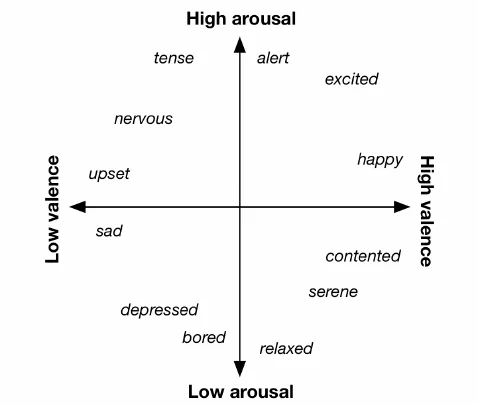
\includegraphics[width=0.60\textwidth]{figures/PAD.png}
    \caption{Proyección bidimensional (Valencia-Arousal) relacionada con modelos dimensionales. El modelo PAD completo incorpora una tercera dimensión (Dominancia) \cite{article}.}
    \label{fig:pad_model}
\end{figure}

Este tipo de representación permite modelar emociones de manera continua y facilita la simulación de cambios emocionales graduales en agentes inteligentes. Además, el modelo PAD ha sido ampliamente utilizado en sistemas de interacción humano-computador, personajes virtuales y agentes conversacionales debido a su simplicidad matemática y flexibilidad computacional.

En muchos modelos afectivos, las emociones evolucionan dinámicamente en función de estímulos internos y externos. Una formulación simplificada de actualización emocional puede expresarse como:

\begin{equation}
Mood_{t+1} = \beta \cdot Mood_t + \alpha \cdot Emotion
\end{equation}

donde $\beta$ representa la persistencia del estado emocional previo y $\alpha$ la influencia del nuevo estímulo emocional sobre el agente.

\subsection{Modelo OCC}

Uno de los modelos más influyentes dentro de la computación afectiva es el modelo OCC (\textit{Ortony, Clore and Collins}), propuesto originalmente para describir la estructura cognitiva de las emociones. Este modelo clasifica las emociones en función de la evaluación cognitiva (\textit{appraisal}) realizada por un individuo sobre eventos, acciones y objetos \cite{occ2009revisited}.

La revisión propuesta por Steunebrink et al. busca resolver algunas ambigüedades presentes en la formulación original de OCC, especialmente en relación con la representación lógica y formal de determinadas emociones complejas \cite{occ2009revisited}.

El modelo OCC organiza las emociones en tres grandes categorías principales:

\begin{itemize}
    \item Emociones relacionadas con las consecuencias de eventos.
    \item Emociones relacionadas con las acciones de agentes.
    \item Emociones relacionadas con aspectos de objetos.
\end{itemize}

A partir de esta estructura, OCC relaciona determinadas evaluaciones cognitivas con emociones concretas. Por ejemplo, el miedo aparece cuando el agente anticipa un evento negativo futuro, mientras que la gratitud surge cuando otro agente realiza una acción considerada beneficiosa.

A pesar de seguir siendo una referencia clásica dentro de la computación afectiva, distintos autores han señalado ciertas ambigüedades en la formalización lógica original de OCC. Steunebrink et al. \cite{occ2009revisited} destacan que algunas categorías emocionales presentan relaciones poco precisas entre eventos, acciones y objetos, dificultando su implementación computacional exacta. Como respuesta, proponen una reinterpretación basada en herencia lógica que clarifica la estructura jerárquica de las emociones y facilita su integración en arquitecturas de agentes inteligentes.

\begin{table}[H]
\centering
\caption{Ejemplos de emociones en el modelo OCC}
\begin{tabular}{|l|l|}
\hline
\textbf{Evaluación cognitiva} & \textbf{Emoción asociada} \\ \hline
Evento deseable & Alegría \\ \hline
Evento indeseable & Malestar \\ \hline
Prospecto deseable & Esperanza \\ \hline
Prospecto indeseable & Miedo \\ \hline
Acción propia aprobable & Orgullo \\ \hline
Acción ajena reprobable & Reproche \\ \hline
Acción ajena beneficiosa & Gratitud \\ \hline
\end{tabular}
\label{tab:occ}
\end{table}

\subsection{Emociones y razonamiento}

Diversos trabajos en neurociencia y psicología cognitiva han mostrado que las emociones influyen directamente sobre procesos racionales y deliberativos. Las emociones afectan a la memoria, la atención selectiva, la evaluación de riesgos y la priorización de objetivos \cite{alfonso2021affect}.

En el contexto de agentes inteligentes, esta relación entre emoción y cognición resulta especialmente relevante en entornos dinámicos e inciertos, donde los agentes deben actuar con recursos limitados y bajo condiciones cambiantes. Incorporar emociones permite reducir espacios de búsqueda, priorizar acciones relevantes y adaptar el comportamiento social de los agentes.

\section{Computación afectiva y agentes emocionales}

La computación afectiva (\textit{Affective Computing}) es un área de investigación interdisciplinar centrada en el desarrollo de sistemas capaces de reconocer, interpretar, modelar y simular emociones humanas. Este campo ha adquirido una gran relevancia dentro de la Inteligencia Artificial, especialmente en aplicaciones relacionadas con interacción humano-computador, robótica social y sistemas multiagente. \cite{picard2000affective}.

El objetivo principal de la computación afectiva no consiste únicamente en representar emociones de manera artificial, sino también en permitir que los sistemas inteligentes adapten su comportamiento en función del estado emocional del entorno o de los usuarios con los que interactúan. De esta manera, los agentes afectivos buscan ajustar sus respuestas según el contexto emocional de la interacción y el estado de los usuarios.

\subsection{Agentes emocionales}

Los agentes emocionales son agentes inteligentes capaces de incorporar estados afectivos dentro de sus procesos internos de razonamiento y toma de decisiones. A diferencia de los agentes puramente racionales, estos sistemas consideran que las emociones pueden modificar prioridades, alterar comportamientos y afectar a la selección de acciones.

En muchos modelos tradicionales de agentes, la toma de decisiones se basa únicamente en objetivos racionales y mecanismos lógicos de planificación. Diversos trabajos en neurociencia y psicología cognitiva muestran que los estados emocionales influyen directamente sobre la atención, la memoria y la toma de decisiones.

La incorporación de emociones permite que los agentes modifiquen prioridades y respuestas en función de cambios producidos durante la interacción. En arquitecturas afectivas como WASABI o EBDI, los estados emocionales pueden modificar prioridades, alterar decisiones o influir sobre la manera en que el agente interactúa con otros usuarios y agentes del entorno.

Además, las emociones permiten representar fenómenos sociales complejos como cooperación, empatía, frustración, culpa o confianza, especialmente relevantes en sistemas multiagente y simulaciones sociales \cite{argente2022normative}.

\subsection{Relación entre emociones y toma de decisiones}

Las emociones influyen directamente sobre numerosos procesos cognitivos humanos, incluyendo percepción, memoria, aprendizaje y razonamiento. En neurociencia, diferentes investigaciones han mostrado que individuos con alteraciones emocionales presentan dificultades significativas en procesos de decisión, incluso cuando mantienen intactas sus capacidades lógicas.

En agentes inteligentes, esta relación entre emoción y razonamiento ha motivado el desarrollo de arquitecturas cognitivas capaces de integrar estados emocionales dentro de los mecanismos deliberativos. Un ejemplo relevante es la arquitectura EBDI, que amplía el modelo BDI clásico incorporando emociones primarias y secundarias en el proceso de toma de decisiones \cite{jiang2007ebdi}.

En la práctica, estos mecanismos permiten que un agente pueda priorizar determinada información, modificar objetivos o seleccionar acciones distintas dependiendo del estado emocional generado durante la interacción. Esto resulta especialmente útil en entornos dinámicos, donde un agente no siempre dispone del tiempo o de la información necesaria para realizar procesos deliberativos complejos.

\subsection{Aplicaciones de la computación afectiva}

La computación afectiva se utiliza actualmente en ámbitos muy diversos, especialmente en sistemas donde la interacción con personas resulta importante. Las aplicaciones de la computación afectiva son muy variadas y dependen del tipo de interacción que el sistema mantiene con usuarios u otros agentes. Algunas de las aplicaciones más habituales son:

\begin{itemize}
    \item \textbf{Asistentes virtuales y agentes conversacionales}: sistemas capaces de detectar emociones del usuario y adaptar sus respuestas.
    
    \item \textbf{Videojuegos y personajes virtuales}: personajes no jugables con comportamientos emocionales dinámicos y realistas.
    
    \item \textbf{Robótica social}: robots diseñados para interactuar socialmente con personas mediante expresiones emocionales.
    
    \item \textbf{Educación inteligente}: tutores virtuales capaces de detectar frustración, aburrimiento o motivación.
    
    \item \textbf{Simulación social}: estudio de dinámicas sociales complejas mediante agentes emocionales.
\end{itemize}

\subsection{Limitaciones actuales}

A pesar de los avances alcanzados, la modelización computacional de emociones continúa siendo un problema abierto. Las emociones humanas poseen un fuerte componente subjetivo, cultural y contextual que resulta difícil de representar mediante modelos computacionales simplificados.

Además, muchos sistemas afectivos actuales utilizan representaciones emocionales limitadas o reducidas, incapaces de capturar completamente la complejidad emocional humana. Otro desafío importante es la validación experimental de los modelos emocionales, ya que evaluar comportamientos afectivos de manera objetiva resulta especialmente complejo.

Por este motivo, gran parte de la investigación actual se centra en desarrollar modelos emocionales más dinámicos, adaptativos y culturalmente conscientes \cite{taverner2021fuzzy,taverner2023multidimensional}; así como arquitecturas capaces de integrar razonamiento cognitivo, emociones y comportamiento social dentro de un mismo sistema inteligente.

Además, muchos modelos actuales siguen dependiendo de conjuntos emocionales relativamente pequeños y simplificados, lo que dificulta representar fenómenos afectivos ambiguos o contradictorios presentes en interacciones humanas reales.

\section{Arquitecturas emocionales para agentes inteligentes}

La incorporación de emociones dentro de agentes inteligentes requiere arquitecturas capaces de integrar razonamiento cognitivo, estados afectivos y comportamiento adaptativo. A lo largo de los años se han desarrollado múltiples propuestas orientadas a combinar procesos deliberativos tradicionales con mecanismos emocionales inspirados en teorías psicológicas y cognitivas.

Muchas de estas arquitecturas parten del modelo BDI (\textit{Beliefs, Desires and Intentions}), ampliamente utilizado en sistemas multiagente debido a su capacidad para representar procesos racionales de decisión. Sin embargo, las limitaciones de los agentes puramente racionales han motivado la aparición de extensiones afectivas capaces de incorporar emociones dentro del razonamiento del agente.

\subsection{Arquitectura BDI}

La arquitectura BDI constituye uno de los modelos cognitivos más utilizados en agentes inteligentes. Este enfoque representa el estado interno de un agente mediante tres componentes fundamentales:

\begin{itemize}
    \item \textbf{Beliefs}: información y conocimiento que el agente posee sobre el entorno.
    
    \item \textbf{Desires}: objetivos o estados que el agente desea alcanzar.
    
    \item \textbf{Intentions}: planes y acciones que el agente decide ejecutar.
\end{itemize}

El proceso deliberativo de un agente BDI consiste en actualizar sus creencias a partir de la percepción del entorno, seleccionar objetivos relevantes y generar intenciones que permitan satisfacer dichos objetivos.

A pesar de su gran utilidad, el modelo BDI tradicional presenta ciertas limitaciones cuando se aplica a entornos sociales complejos o interacciones humanas. En particular, este modelo asume un comportamiento fundamentalmente racional, ignorando el papel que desempeñan las emociones en la toma de decisiones humanas.

Como consecuencia, numerosos trabajos han propuesto extensiones emocionales del modelo BDI orientadas a incorporar estados afectivos dentro del razonamiento deliberativo.

\subsection{Arquitectura EBDI}

Una de las extensiones más conocidas del modelo BDI es la arquitectura EBDI (\textit{Emotional Belief-Desire-Intention}), propuesta para integrar emociones dentro del ciclo cognitivo de los agentes. En esta arquitectura, las emociones actúan como mecanismos capaces de priorizar creencias, modificar objetivos y filtrar decisiones en entornos dinámicos. Jiang et al. distinguen además entre emociones primarias, asociadas a respuestas rápidas, y emociones secundarias, relacionadas con procesos deliberativos más complejos \cite{jiang2007ebdi}.

\begin{figure}[H]
    \centering
    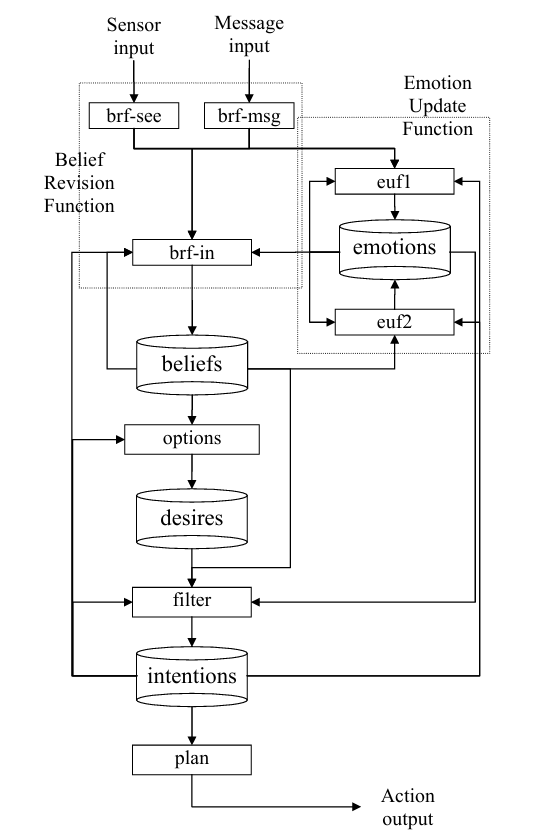
\includegraphics[width=0.62\textwidth]{figures/ebdi_architechture.png}
    \caption{Arquitectura EBDI para agentes emocionales \cite{jiang2007ebdi}.}
    \label{fig:ebdi_architecture}
\end{figure}

Como se observa en la figura  \ref{fig:ebdi_architecture}, las emociones se incorporan como un componente adicional que influye directamente sobre la selección de objetivos, la priorización de planes y la toma de decisiones. De esta forma, el comportamiento del agente no depende únicamente de procesos racionales, sino también de su estado emocional actual.

La arquitectura EBDI utiliza mecanismos inspirados en teorías de appraisal para generar emociones a partir de eventos percibidos por el agente. Estas emociones pueden clasificarse en emociones primarias y secundarias, dependiendo del nivel de procesamiento cognitivo asociado.

Una de las principales aportaciones de EBDI es la separación entre el mecanismo emocional y el proceso de razonamiento práctico del agente \cite{jiang2007ebdi}. Esta separación permite incorporar distintos modelos emocionales sin modificar el núcleo deliberativo de la arquitectura. Además, el modelo distingue entre emociones primarias y secundarias: las emociones primarias actúan como un mecanismo rápido de priorización de creencias y decisiones en entornos dinámicos o con recursos limitados, mientras que las emociones secundarias refinan el razonamiento cuando existe mayor capacidad deliberativa.

De forma simplificada, el ciclo de funcionamiento de un agente EBDI puede describirse mediante las siguientes etapas:

\begin{enumerate}
    \item Percepción del entorno.
    \item Actualización de creencias.
    \item Evaluación emocional de eventos.
    \item Generación de deseos e intenciones.
    \item Selección de acciones.
\end{enumerate}

Esto permite que el agente no actúe únicamente siguiendo objetivos racionales fijos, sino que pueda modificar prioridades dependiendo de la situación emocional percibida.

\subsection{Arquitectura WASABI}

La arquitectura WASABI destaca especialmente por su orientación hacia humanos virtuales expresivos e interacción social creíble \cite{becker2009wasabi}. El sistema combina razonamiento cognitivo con simulación continua de estados afectivos dentro del espacio PAD, permitiendo representar cambios emocionales continuos durante la interacción.

El artículo utiliza como caso de estudio el humano virtual MAX, evaluado en un escenario interactivo basado en un juego de cartas. Además de emociones primarias relacionadas con respuestas rápidas y expresivas, WASABI incorpora emociones secundarias como esperanza (\textit{hope}), alivio (\textit{relief}) y miedo confirmado (\textit{fears-confirmed}), asociadas a procesos cognitivos más complejos y expectativas futuras.

Según los resultados presentados en el artículo, los usuarios percibían al agente como más coherente durante la interacción cuando las emociones secundarias se combinaban con la simulación emocional continua.

En este modelo, las emociones se representan mediante espacios tridimensionales continuos:

\begin{equation}
E = (P, A, D)
\end{equation}

donde:

\begin{itemize}
    \item $P$ representa Pleasure.
    \item $A$ representa Arousal.
    \item $D$ representa Dominance.
\end{itemize}

A diferencia de EBDI, cuyo objetivo principal es integrar emociones dentro del razonamiento deliberativo de agentes racionales, WASABI se centra especialmente en la expresividad emocional y en la percepción de realismo durante la interacción humano-agente. Esta orientación hacia humanos virtuales hace que WASABI sea especialmente relevante para aplicaciones relacionadas con simulación social, personajes virtuales y sistemas de interacción humano-computador capaces de mantener respuestas afectivas más consistentes durante la interacción.

\subsection{Modelos afectivos modernos}

En los últimos años han surgido nuevas propuestas orientadas a integrar emociones, cognición, memoria y comportamiento social dentro de arquitecturas más flexibles e integradas \cite{alfonso2021affect}.

Muchos de estos modelos buscan combinar mecanismos emocionales con memoria, aprendizaje y adaptación social. El objetivo es superar las limitaciones de arquitecturas más rígidas, donde las emociones suelen representarse mediante conjuntos estáticos o respuestas predefinidas.

Asimismo, investigaciones recientes exploran la utilización de modelos híbridos que combinan representación simbólica, lógica difusa, aprendizaje automático y sistemas probabilísticos para mejorar la simulación emocional en agentes inteligentes.

El auge reciente de asistentes conversacionales y sistemas generativos ha incrementado el interés por arquitecturas capaces de representar estados afectivos de manera más flexible y dinámica.

\subsection{Comparación entre arquitecturas}

Las distintas arquitecturas emocionales presentan enfoques diferentes respecto a la representación emocional, el razonamiento afectivo y la toma de decisiones.

\begin{table}[H]
\centering
\caption{Comparación entre arquitecturas emocionales}
\small
\begin{tabular}{|l|l|l|l|}
\hline
\textbf{Arquitectura} & \textbf{Modelo} & \textbf{Representación} & \textbf{Aplicaciones} \\ \hline
BDI & No emocional & Simbólica & Agentes racionales \\ \hline
EBDI & Appraisal & Modular / dependiente del modelo & Agentes deliberativos \\ \hline
WASABI & PAD & Dimensional continua & Humanos virtuales \\ \hline
Modelos modernos & Híbrido & Mixta & IA social avanzada \\ \hline
\end{tabular}
\label{tab:comparacion}
\end{table}

Cada arquitectura presenta ventajas y limitaciones dependiendo del tipo de aplicación y del nivel de complejidad emocional requerido. Mientras que modelos discretos como OCC facilitan la interpretación semántica de emociones específicas, los enfoques dimensionales permiten representar transiciones emocionales más suaves y dinámicas.

Actualmente, la tendencia principal en computación afectiva consiste en desarrollar arquitecturas híbridas capaces de integrar razonamiento cognitivo, representación emocional continua y adaptación social dentro de sistemas inteligentes complejos.

\section{Representación computacional de emociones}

Uno de los principales desafíos dentro de la computación afectiva consiste en representar emociones de forma computacional. A diferencia de otros procesos cognitivos más estructurados, las emociones poseen características subjetivas, dinámicas y dependientes del contexto, lo que dificulta su modelado mediante técnicas tradicionales de Inteligencia Artificial.

A lo largo de los años se han desarrollado distintos enfoques orientados a representar estados emocionales dentro de agentes inteligentes. Estas representaciones pueden clasificarse principalmente en modelos discretos, dimensionales e híbridos.

\subsection{Representación discreta de emociones}

Los modelos discretos representan las emociones como categorías diferenciadas y semánticamente interpretables. Este enfoque se basa generalmente en teorías psicológicas que consideran la existencia de emociones básicas universales.

Uno de los modelos más utilizados en computación afectiva es el modelo OCC, donde emociones como alegría, miedo, orgullo o vergüenza se generan a partir de procesos de evaluación cognitiva (\textit{appraisal}) asociados a eventos, acciones u objetos \cite{occ2009revisited}.

La principal ventaja de los modelos discretos consiste en su interpretabilidad semántica, ya que cada emoción posee un significado claramente definido. Esto facilita la implementación de comportamientos emocionales comprensibles en agentes conversacionales, personajes virtuales y sistemas interactivos.

Sin embargo, este enfoque presenta ciertas limitaciones relacionadas con la dificultad para representar transiciones emocionales graduales o estados afectivos ambiguos.

\subsection{Representación dimensional}

Los modelos dimensionales representan emociones mediante espacios continuos definidos por distintas dimensiones emocionales. Este enfoque permite modelar emociones como combinaciones de variables numéricas continuas, facilitando la simulación de cambios emocionales dinámicos.

Uno de los modelos dimensionales más utilizados es PAD (\textit{Pleasure-Arousal-Dominance}), donde cada estado emocional se representa mediante tres dimensiones principales:

\begin{equation}
E = (P, A, D)
\end{equation}

donde:

\begin{itemize}
    \item $P$ representa el nivel de placer o desagrado.
    \item $A$ representa el nivel de activación emocional.
    \item $D$ representa el grado de dominancia o control.
\end{itemize}

Este tipo de representación permite describir emociones complejas mediante posiciones dentro de un espacio continuo multidimensional. Por ejemplo, emociones como entusiasmo presentan valores altos de placer y activación, mientras que tristeza se asocia normalmente a valores bajos de activación y placer.

Los modelos dimensionales resultan especialmente útiles en sistemas dinámicos, personajes virtuales y simulaciones sociales, ya que permiten representar transiciones emocionales suaves y continuas.

\subsection{Lógica difusa y emociones}

Debido a la naturaleza subjetiva e imprecisa de las emociones humanas, numerosos trabajos han incorporado técnicas de lógica difusa (\textit{Fuzzy Logic}) para modelar incertidumbre emocional y grados de intensidad afectiva.

En estos modelos, las emociones no se representan como estados absolutos, sino mediante funciones de pertenencia que indican el grado en que un agente experimenta una determinada emoción.

Una representación simplificada de pertenencia difusa puede expresarse mediante:

\begin{equation}
\mu_{fear}(x) \in [0,1]
\end{equation}

donde $\mu_{fear}(x)$ representa el grado de intensidad asociado a la emoción de miedo ante una determinada situación.

Diversos trabajos recientes han utilizado sistemas difusos para combinar evaluación cognitiva (\textit{appraisal}), intensidad emocional y adaptación contextual. Por ejemplo, modelos orientados a entornos multiculturales emplean reglas de inferencia difusa para evaluar eventos y generar emociones imprecisas, las cuales son posteriormente convertidas mediante un proceso de defuzzificación y proyectadas sobre dimensiones continuas como el Placer y el Arousal \cite{taverner2021fuzzy}.

\subsection{Representación cultural de emociones}

Uno de los problemas más relevantes en computación afectiva es la influencia cultural sobre la interpretación y expresión emocional. Diferentes culturas pueden expresar, percibir y valorar emociones de manera distinta, lo que dificulta la construcción de modelos emocionales universales.

Investigaciones recientes han propuesto modelos multidimensionales culturalmente adaptados capaces de modificar la representación emocional en función del contexto sociocultural \cite{taverner2023multidimensional}.

Estos modelos permiten modificar distintos parámetros emocionales dependiendo del contexto sociocultural, incluyendo intensidad afectiva, interpretación contextual y valoración social de determinadas emociones.

La incorporación de adaptación cultural resulta especialmente importante en sistemas conversacionales globales, simulaciones sociales y agentes virtuales diseñados para interactuar con usuarios de diferentes entornos culturales.

\subsection{Modelos híbridos}

Actualmente, muchos sistemas afectivos utilizan modelos híbridos que combinan representaciones discretas, dimensionales y difusas con el objetivo de aprovechar las ventajas de cada enfoque.

Por ejemplo, arquitecturas híbridas como WASABI \cite{becker2009wasabi} pueden utilizar un appraisal cognitivo para generar emociones discretas (diferenciando entre primarias y secundarias), mientras que posteriormente emplean espacios dimensionales PAD para representar la intensidad y la evolución continua del estado de ánimo.

Asimismo, algunos modelos modernos integran técnicas de aprendizaje automático y representación probabilística para adaptar dinámicamente los estados emocionales del agente en función de la experiencia y del entorno.

Por este motivo, muchos trabajos recientes apuestan por enfoques híbridos capaces de combinar representación simbólica, espacios dimensionales y aprendizaje adaptativo dentro de un mismo sistema.

\section{Normas sociales y emociones en sistemas multiagente}

Diversas emociones sociales influyen directamente en el comportamiento social humano. Emociones como culpa, vergüenza, empatía o aprobación social influyen directamente sobre la cooperación, el cumplimiento de normas y la toma de decisiones colectivas.

En sistemas multiagente, diferentes investigaciones han explorado la integración de emociones sociales dentro de arquitecturas normativas con el objetivo de modelar comportamientos más flexibles y socialmente consistentes \cite{argente2022normative}.

Los agentes normativos emocionales combinan mecanismos tradicionales de razonamiento con estados afectivos capaces de modificar el comportamiento del agente en función del contexto social. De esta forma, las emociones actúan como mecanismos reguladores que afectan tanto al cumplimiento de normas como a las interacciones entre agentes.

Por ejemplo, emociones negativas como culpa o vergüenza pueden aumentar la probabilidad de que un agente respete determinadas normas sociales, mientras que emociones positivas como orgullo o aprobación social pueden reforzar comportamientos cooperativos.

\begin{table}[H]
\centering
\caption{Ejemplos de emociones sociales en agentes normativos}
\begin{tabular}{p{4cm} p{8cm}}
\toprule
\textbf{Emoción} & \textbf{Efecto sobre el agente} \\
\midrule
Culpa & Incrementa cumplimiento normativo \\
Vergüenza & Reduce conductas socialmente negativas \\
Orgullo & Refuerza cooperación y reputación \\
Empatía & Favorece colaboración entre agentes \\
\bottomrule
\end{tabular}
\end{table}

La incorporación de emociones sociales resulta especialmente relevante en aplicaciones relacionadas con simulación social, negociación automática, robótica social y sistemas colaborativos.

Sin embargo, la modelización de normas sociales y emociones continúa siendo un problema complejo debido a la fuerte dependencia contextual y cultural de este tipo de comportamientos.

\section{Discusión y retos actuales}

La incorporación de emociones dentro de agentes inteligentes ha permitido desarrollar sistemas más adaptativos, creíbles y socialmente coherentes. A lo largo de los últimos años, la computación afectiva ha evolucionado desde modelos emocionales simples hasta arquitecturas complejas capaces de integrar razonamiento cognitivo, emociones y comportamiento social.

Sin embargo, su representación computacional continúa presentando importantes limitaciones. La fuerte dependencia contextual, cultural y subjetiva del afecto humano resulta difícil de modelar mediante representaciones simplificadas. De hecho, muchos sistemas actuales utilizan conjuntos limitados de emociones o mecanismos estáticos, lo que reduce la naturalidad del agente. A esto se suma la complejidad de la validación experimental, ya que evaluar si un agente expresa emociones de manera realista y coherente sigue siendo un problema abierto en la Inteligencia Artificial social.

En general, las líneas de investigación actuales buscan desarrollar agentes capaces de mantener estados emocionales más coherentes a largo plazo, integrar aprendizaje y memoria afectiva, y adaptarse de manera flexible a distintos contextos sociales y culturales.

\subsection{Relación entre los trabajos analizados}

Los trabajos estudiados representan diferentes etapas dentro de la evolución de los agentes afectivos. El modelo OCC proporciona una estructura cognitiva para generar emociones mediante procesos de appraisal, mientras que arquitecturas como EBDI integran dichas emociones dentro del razonamiento deliberativo de agentes BDI.

Por otro lado, WASABI extiende estos enfoques hacia humanos virtuales capaces de representar dinámicas emocionales continuas mediante el modelo PAD. Asimismo, los trabajos de Taverner et al. incorporan representación difusa y adaptación cultural, resolviendo algunas limitaciones presentes en modelos emocionales puramente discretos.

Desde nuestro punto de vista, cada enfoque presenta ventajas y limitaciones diferentes. OCC resulta especialmente útil por su interpretabilidad semántica y su facilidad para relacionar emociones con procesos de appraisal, aunque los modelos discretos presentan dificultades para representar intensidad y evolución temporal de manera continua. Por otro lado, modelos dimensionales como PAD permiten describir transiciones emocionales más suaves, pero sacrifican parte de la interpretación semántica directa de cada emoción. Arquitecturas como EBDI integran emociones dentro de la toma de decisiones, mientras que WASABI destaca especialmente en contextos orientados a interacción y expresividad emocional.

Finalmente, los agentes normativos emocionales amplían estas arquitecturas hacia entornos sociales y multiagente, donde emociones como culpa, empatía o vergüenza influyen directamente sobre el comportamiento cooperativo y el cumplimiento de normas.

En definitiva, la computación afectiva está adquiriendo un papel cada vez más relevante dentro de la Inteligencia Artificial social.

\section{Conclusiones}

La incorporación de emociones dentro de agentes inteligentes constituye una de las principales líneas de investigación en computación afectiva y sistemas multiagente. A través de distintos modelos psicológicos y arquitecturas cognitivas, numerosos trabajos han demostrado que las emociones pueden mejorar significativamente la adaptación, interacción y comportamiento social de los agentes artificiales.

En este trabajo se han revisado los principales enfoques utilizados para representar emociones computacionalmente, incluyendo modelos discretos, dimensionales e híbridos. Asimismo, se han analizado arquitecturas afectivas como EBDI y WASABI, así como propuestas relacionadas con emociones sociales y sistemas multiagente normativos.

A pesar de los avances alcanzados, continúan existiendo importantes desafíos relacionados con la subjetividad emocional, la adaptación cultural y la integración entre emoción, cognición y aprendizaje.

El creciente desarrollo de agentes conversacionales avanzados y sistemas de Inteligencia Artificial social hace prever que la computación afectiva seguirá adquiriendo una gran relevancia en los próximos años, especialmente en aplicaciones relacionadas con interacción humano-computador, robótica social y simulación social inteligente.

% ------------------------------------------------
%                BIBLIOGRAPHY
% ------------------------------------------------

\newpage

\nocite{*}
\printbibliography

\end{document}